%\documentstyle[epsf,twocolumn]{jarticle}       %LaTeX2.09仕様
%\documentclass[twocolumn]{jarticle}     %pLaTeX2e仕様
\documentclass{jarticle}     %pLaTeX2e仕様

%一枚組だったら[twocolumn]関係のとこ消す

\setlength{\topmargin}{-45pt}
%\setlength{\oddsidemargin}{0cm} 
\setlength{\oddsidemargin}{-7.5mm}
%\setlength{\evensidemargin}{0cm} 
\setlength{\textheight}{24.1cm}
%setlength{\textheight}{25cm} 
\setlength{\textwidth}{17.4cm}
%\setlength{\textwidth}{172mm} 
\setlength{\columnsep}{11mm}

\kanjiskip=.07zw plus.5pt minus.5pt

\usepackage{graphicx}
\usepackage[dvipdfmx]{color}
\usepackage{subcaption}
\usepackage{enumerate}
\usepackage{comment}
\usepackage{url}
\usepackage{multirow}
\usepackage{diagbox}
\usepackage{amsmath,amssymb}
\usepackage{mathtools}
\usepackage{wrapfig}
\usepackage{graphicx}
\usepackage{float}
\usepackage{algorithmic}
\usepackage{algorithm}


\begin{document}

  \noindent
  \hspace{1em}

  \today
  \hfill
  \ \  B3 西村昭賢 

  \vspace{2mm}
  \hrule
  \begin{center}
  {\Large \bf 進捗報告}
  \end{center}
  \hrule
  \vspace{3mm}


\section{今週やったこと}
\begin{quote}
  \begin{itemize}
   \item 研究発表会の準備(スライド)
   \item ゲームバランス調整のアプローチ検討
   \item 自作環境の改良 \& ルール確定
   \item エージェント作成実験
  \end{itemize}
 \end{quote}

\section{ゲームバランス調整について}
構築環境への強化学習手法の適用を研究の目的の1つとしたため,強化学習で作成したエージェントを用いてバランス調整を行いたいと考えた.\par
インターンでゲーム開発現場においてパラメータチューニングが属人化しやすいという話を聞いたので,バランス調整ではカードのHP,攻撃力を調整することにする.
現在は図 \ref{fig:idea} のようなアプローチを考えている.

\begin{quote}
  \begin{itemize}
   \item 良いと考えている点
   \par
   \begin{quote}
    \begin{itemize}
     \item 強化学習でルールベースAIに勝つような戦略を持つAIを作成することでより実践的なシミュレーションが行える.
     \item 調整したいデッキを用意することで自動で行える
    \end{itemize}
   \end{quote}
   \item 良くないと考えている点
   \par
   \begin{quote}
    \begin{itemize}
     \item 深層強化学習を用いると学習に時間がかかる
     \item ルールベースに勝つように学習するためルールベースで作成したAIに大きく依存する
    \end{itemize}
   \end{quote}
  \end{itemize}
 \end{quote}

 各カードの戦績の計算に用いる指標としては,
 \begin{quote}
  \begin{itemize}
   \item 盤面に出されてから生きているターン数
   \item 倒した敵カードの数
   \item 敵プレイヤーに与えたダメージ
  \end{itemize}
 \end{quote}
 を考えている.
 また, HearthStone のバランス調整を試した研究\cite{HearthStone}では Win Rate when Played (WRP) , Win Rate when Drawed (WPD) という指標を用いられている.\par
 まだ考えがまとまっていないが,強化学習の学習済みエージェントでシミュレーションすることでより実践的な対戦データを得られるためバランス調整に生かせそうと考えている.



\begin{figure}[H]
  \centering
  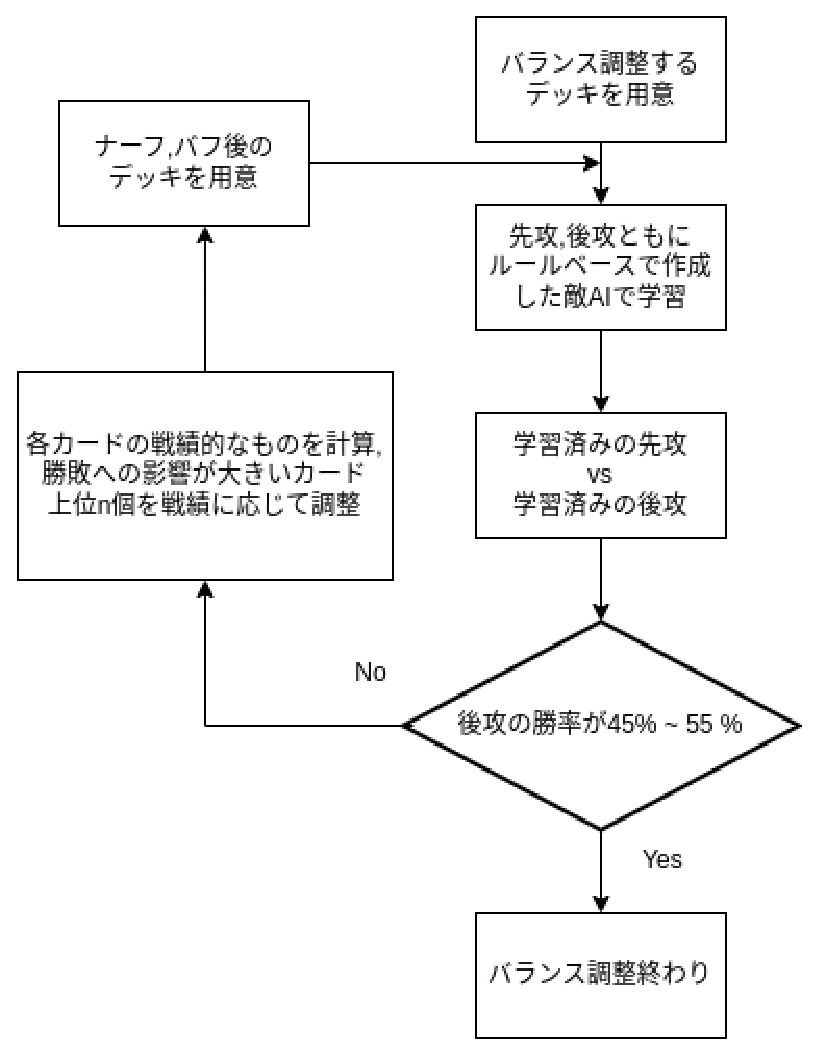
\includegraphics[width=120mm]{assets/ideaimage.eps}
  \caption{バランス調整アイデア}
  \label{fig:idea}
\end{figure}

\section{自作環境の改良 \& ルール確定}
バランス調整に取り掛かるにあたって,先週までのルールはコストがなくカードのプレイに関して戦略性がないルールになっていた.
より一般的な TCG に寄せたルールのゲームを作成し, 構築環境として確定しバランス調整に取り組みたいと考えた.追加した点をいかに述べる.
\begin{quote}
  \begin{itemize}
   \item プレイヤー
   \par
   \begin{quote}
    \begin{itemize}
     \item HP
     \par
     最大 20, 0 となればゲーム敗北
     \item マナコスト
     \par
     ゲーム開始時1 , 最大 5 , ターンごとに 1 増加
     \item ライブラリ
     \par
     ライブラリは30枚のカードを持つ
    \end{itemize}
   \end{quote}
   \item カード
   \begin{quote}
    \begin{itemize}
     \item コスト
     \par
     盤面にプレイする際にカードのコスト分プレイヤーのマナコスト減少
     \item 特殊効果
     \par
     \begin{quote}
      \begin{itemize}
       \item 盤面に出したら (攻撃力 , HP) = ( 1 , 1 )のユニット追加で出す. (召喚)
       \item 盤面に出したら自プレイヤーの HP を 2 回復 (治癒)
       \item 盤面に出したら敵プレイヤーの HP を 2 削る (攻撃)
       \item 盤面に出したら自プレイヤーは 1 枚カードをドロー (循環)
       \item 盤面に出たターンに攻撃できる (速攻)
      \end{itemize}
     \end{quote}
    \end{itemize}
   \end{quote}
   \item 終了条件
   \par
   どちらかのプレイヤーの体力が 0 以下となった ,または デッキ切れの状態でドローしようとした時

  \end{itemize}
 \end{quote}



\section{実験}
強化学習が適用できるか実験を行った.
\subsection{行動空間と状態空間の定義}
環境の改変により定義し直した状態空間と行動空間は表 \ref{table:state} , \ref{table:action} に示す.
\begin{table}[H]
  \centering
  \caption{定義した状態空間 (太字は新しく追加したパラメータ)}
  \label{table:state}
  \begin{tabular}{|c|c|c|c|}
  \hline
  状態説明                        & 次元数        & 最小値        & 最大値         \\ \hline
  \textbf{自,敵プレイヤーのHP}  & \textbf{2} & \textbf{0} & \textbf{20} \\
  \hline
  \textbf{自,敵プレイヤーのコスト} & \textbf{2} & \textbf{0} & \textbf{5} \\ \hline

  手札 1 $\sim$9 の HP と攻撃力      & 18         & 0          & 20          \\ \hline
  \textbf{手札 1 $\sim$ 9 のコスト} & \textbf{9} & \textbf{0} & \textbf{5} \\ \hline
  \textbf{手札 1 $\sim$ 9 の特殊効果} &  \textbf{9} & \textbf{0} & \textbf{5} \\ \hline
  自盤面 1 $\sim$ 5 の HP と攻撃力     & 10         & 0          & 20          \\ \hline
  敵盤面 1 $\sim$ 5 の HP と攻撃力     & 10         & 0          & 20          \\ \hline
  自盤面 1 $\sim$ 5 がターン中行動可能かどうか & 5          & 0          & 1           \\ \hline
  お互いのライブラリの残り枚数     & 2 & 0 & 15 \\ \hline
  \end{tabular}
  \end{table}

  \begin{table}[H]
    \centering
    \caption{定義した行動空間(太字は今回新規に追加したパラメータ)}
    \label{table:action}
    \begin{tabular}{|c|c|}
    \hline
    行動説明                          & 次元数        \\ \hline
    手札1$\sim$9を自盤面に出す             & 9          \\ \hline
    手札1$\sim$9を自盤面に出さない & 9 \\ \hline
    自盤面1が敵盤面1$\sim$5に攻撃or何もしないor\textbf{敵プレイヤーに攻撃}    & \textbf{7}          \\ \hline
    自盤面2が敵盤面1$\sim$5に攻撃or何もしないor\textbf{敵プレイヤーに攻撃}    & \textbf{7}   \\ \hline
    自盤面3が敵盤面1$\sim$5に攻撃or何もしないor\textbf{敵プレイヤーに攻撃}    & \textbf{7}\\ \hline
    自盤面4が敵盤面1$\sim$5に攻撃or何もしないor\textbf{敵プレイヤーに攻撃}    & \textbf{7} \\ \hline
    自盤面5が敵盤面1$\sim$5に攻撃or何もしないor\textbf{敵プレイヤーに攻撃}    & \textbf{7}\\ \hline
    \end{tabular}
    \end{table}
  
\subsection{ライブラリ}
プレイヤーのライブラリは先攻と後攻同じものとした.
デッキの詳細を表 \ref{table:deck} に示す.

\begin{table}[H]
  \centering
  \caption{ライブラリ ()内の数字は(攻撃力, HP, コスト)を表す}
  \label{table:deck}
  \begin{tabular}{|c|c|c|c|c|}
  \hline
  攻撃力 & HP & コスト & 特殊効果 & 枚数 \\ \hline
  1 & 1 & 0 & 無し & 2 \\ \hline
  2 & 1 & 1 & 無し & 2 \\ \hline
  3 & 2 & 2 & 無し & 2 \\ \hline
  4 & 3 & 3 & 無し & 2 \\ \hline
  5 & 4 & 4 & 無し & 2 \\ \hline
  2 & 2 & 2 & 召喚 & 2 \\ \hline
  2 & 3 & 3 & 召喚 & 2 \\ \hline
  1 & 1 & 1 & 循環 & 2 \\ \hline
  1 & 3 & 2 & 循環 & 2 \\ \hline
  2 & 1 & 2 & 速攻 & 2 \\ \hline
  3 & 1 & 3 & 速攻 & 2 \\ \hline
  1 & 2 & 2 & 攻撃 & 2 \\ \hline
  2 & 3 & 3 & 攻撃 & 2 \\ \hline
  1 & 1 & 1 & 治癒 & 2 \\ \hline
  2 & 1 & 3 & 治癒 & 2 \\ \hline
  \end{tabular}
  \end{table}

\subsection{DQNのパラメータ}
DQNのパラメータを表 \ref{table:updateparam} に示す.ε-greedy について学習が進むに連れて学習率が減少していくように変更した.
\begin{table}[H]
  \centering
  \caption{DQNのパラメータ}
  \label{table:updateparam}
  \begin{tabular}{|c||c|}
  \hline
  方策                 & ε-greedy \\ \hline
  εの初期値                      & 1.0      \\ \hline
  εの最小値                      & 0.1      \\ \hline
  εの推移                      & (学習ステップ数 / 3) ステップまで線形的に減少      \\ \hline       
  全結合層の活性化関数             & ReLU     \\ \hline
  全結合層の次元                & 64       \\ \hline
  最適化アルゴリズム              & Adam     \\ \hline
  Target Network 更新重み              & 0.5     \\ \hline
  Exprience Memory への書き込み開始step & 10000 \\ \hline
  Experience Replayのメモリ量 & 50000  \\ \hline
  \end{tabular}
  \end{table}
\subsection{敵プレイヤーの行動}
ルールベースである程度強いAI相手と学習させたかったので以下のような行動ルーチンとした.

\begin{figure}[H]
  \begin{algorithm}[H]
      \caption{敵の行動}
      \label{alg1}
      \begin{algorithmic}[1] 
      \FOR{手札のカード}
      \IF{盤面にプレイできる}
      \STATE カードをプレイ
      \ELSE
      \STATE pass
      \ENDIF
      \ENDFOR
      \FOR{自盤面のカード}
      \IF{敵の盤面に 1 会の攻撃で倒せるカードがある}
      \STATE そのカードを選んで攻撃
      \ELSE
      \STATE 敵プレイヤーを攻撃
      \ENDIF
      \ENDFOR
      \end{algorithmic}
  \end{algorithm}
  \end{figure}
要するに手札から出せる分出して, 敵盤面に倒せるカードがあればカードを攻撃, なければ敵プレイヤーを攻撃するという攻撃的な行動になっている.
この敵を対象に DQN で 先攻プレイヤーを 1000000 ステップ学習を行い, 学習済みモデルで 10000 回対戦を行い勝率を計算した.

\subsection{報酬}
報酬は (\ref{reward}) 式 のように設定した.
\begin{equation}
  \label{reward}
  reward = 0.0,
  \quad 
  \mathrm{1 エピソード終了後}
  reward \text{ = }
  \left\{
    \begin{aligned}
        1.0 \quad & (学習プレイヤーの勝利) \\
        -1.0 \quad & (敵プレイヤーの勝利) \\
    \end{aligned}
    \right.
\end{equation}


\subsection{結果と考察}
実験結果を表 \ref{table:jikken} に示す.また,図 に学習中の DQN の 200 エピソード中の獲得報酬平均の推移を示す
\begin{table}[H]
  \centering
  \caption{実験の結果}
  \label{table:jikken}
  \begin{tabular}{|c|c|}
  \hline
  手法 & 勝率     \\ \hline
  敵プレイヤーと同じ行動      & \textbf{0.5033}  \\ \hline
  DQN      & 0.1461 \\ \hline
  \end{tabular}
  \end{table}

  \begin{figure}[H]
    \centering
    \includegraphics[width=120mm]{assets/DQNreward.eps}
    \caption{DQN学習中における獲得報酬平均の推移}
    \label{fig:DQN}
  \end{figure}

結果としては DQN で 1 割程度の勝率しか得ることができなかった.
学習が上手く進まなかった原因として以下の要因が考えられる.

\begin{quote}
  \begin{itemize}
   \item 学習ステップ数不足
   \par
   今回の実験では対戦相手がルールベースの AI であり reward が 1 となるエピソードが少ない.そのため学習が上手く進まなかったと考えられる.今回はゼミに間に合わせるために 1000000ステップ,約 22000 エピソード学習を行ったが, ステップ数を増やして実験を試してみる.
   \item reward の与え方
   \par
   一般的な TCG の勝利条件は相手のプレイヤーの HP を 0 にする, または相手がデッキ切れ起こすことであり,今回作成した環境でも同じ勝利条件を採用した.
   よく考えてみると相手のプレイヤーの HP を 0 にするようにはある程度攻撃的に行動しなければならず, 相手のデッキ切れを誘うには防戦的に動く必要がある.
   \par
   今回の実験では reward を 勝利すれば 1.0 としていたため学習側プレイヤーの戦略が学習により上手く構築できなかったのではないかと考えた. 例えば相手の HP を 0にしたら reward = 1.0, 相手のデッキ切れで勝ったら reward = 0.1 など重みをつけたら学習の進み具合が変わるかもしれない.
  \end{itemize}
 \end{quote}

\section{わからんこと}
今回, DQN で ε-greedy の ε を最初は 1.0 として 0.1 に収束させる方法を採用したのですが,εの減少の方法が調べてもあまり見つかりませんでした. 今回の実験では (学習ステップ数 / 3) ステップまで線形的に減少としましたが ,なにか良い方法があればご教授いただければ幸いです.

\section{今後やること}
\begin{quote}
  \begin{itemize}
   \item 研究発表会の準備(資料作成)
   \item ゲームバランス調整のアプローチ検討
   \item 改良した構築環境への強化学習適用
   \par
   先週までのゲームルールから戦略性, ゲーム性を増したいだけなのでプレイヤーの HP 有りで上手く行かなかったら HP 無しに切り替える予定. なるべく HP 有りでやってみたいので今週はいろいろ検討してみる.
  \end{itemize}
 \end{quote}

%index.bibはtexファイルと同階層に置く
%ちゃんと\citeしないと表示されない(1敗)
\bibliography{index.bib}
\bibliographystyle{junsrt}

\end{document}